


%% LyX 2.2.3 created this file.  For more info, see http://www.lyx.org/.
%% Do not edit unless you really know what you are doing.
\documentclass[english]{article}
\usepackage[latin9]{inputenc}
\usepackage{geometry}
\geometry{verbose,tmargin=0.8in,bmargin=0.8in,lmargin=1in,rmargin=1in,headheight=0cm,headsep=0cm}
\usepackage{babel}
%\usepackage[unicode=true]
\usepackage{listings}
\usepackage{color}

\definecolor{dkgreen}{rgb}{0,0.6,0}
\definecolor{gray}{rgb}{0.5,0.5,0.5}
\definecolor{mauve}{rgb}{0.58,0,0.82}

\lstset{frame=tb,
  language=Java,
  aboveskip=3mm,
  belowskip=3mm,
  showstringspaces=false,
  columns=flexible,
  basicstyle={\small\ttfamily},
  numbers=none,
  numberstyle=\tiny\color{gray},
  keywordstyle=\color{blue},
  commentstyle=\color{dkgreen},
  stringstyle=\color{mauve},
  breaklines=true,
  breakatwhitespace=true,
  tabsize=3
}
\usepackage{graphicx}
% {hyperref}
\makeatletter
%%%%%%%%%%%%%%%%%%%%%%%%%%%%%% LyX specific LaTeX commands.
%% Because html converters don't know tabularnewline
\providecommand{\tabularnewline}{\\}

\makeatother

\begin{document}
\begin{center}
{\Large{}CSCE 221 Cover Page}\\
{\Large{} Homework Assignment \#2 }\\
{\Large{}Due March 25 at 23:59 pm to eCampus}
\par\end{center}{\Large \par}

\begin{flushright}
{\Large{}First Name~~Hunter~~~Last Name~~Cleary~~~~~~UIN~~625001547~~~}
\par\end{flushright}{\Large \par}

\begin{flushright}
{\Large{}User Name ~~hncleary~~~~~E-mail address~~hncleary@tamu.edu~~~}\medskip{}
\par\end{flushright}
\begin{quotation}
Please list all sources in the table below including web pages which
you used to solve or implement the current homework. If you fail to
cite sources you can get a lower number of points or even zero, read
more Aggie Honor System Office \href{http://aggiehonor.tamu.edu/}{http://aggiehonor.tamu.edu/}\medskip{}
\medskip{}
\end{quotation}
\begin{tabular}{|c|c|c|c|}
\hline 
Type of sources  & ~~~~~~~~~~~~~~~~~~~~~~~ & ~~~~~~~~~~~~~~~~~~~~~~~~ & ~~~~~~~~~~~~~~~~~~~~~~~\tabularnewline
 &  &  & \tabularnewline
\hline 
\hline 
People &  &  & \tabularnewline
 &  &  & \tabularnewline
\hline 
Web pages (provide URL)  &Links Below  &  & \tabularnewline
 &  &  & \tabularnewline
\hline 
Printed material & Data Structures and Algorithms  &  & \tabularnewline
 &(Textbook) &  & \tabularnewline
\hline 
Other Sources  &  &  & \tabularnewline
 &  &  & \tabularnewline
\hline 
\end{tabular}\ \\ \ \\
https://en.wikipedia.org/wiki/Master\_theorem\_(analysis\_of\_algorithms)\ \\
https://www.geeksforgeeks.org/quick-sort/\ \\
https://www.geeksforgeeks.org/merge-sort/\ \\
https://en.wikipedia.org/wiki/Skip\_list\ \\
http://www.cplusplus.com/reference/queue/queue/\ \\
https://www.cs.auckland.ac.nz/software/AlgAnim/AVL.html\ \\
https://en.wikipedia.org/wiki/Recurrence\_relation

\medskip{}
\medskip{}
\begin{quotation}
I certify that I have listed all the sources that I used to develop
the solutions/codes to the submitted work.

\textquotedblleft On my honor as an Aggie, I have neither given nor
received any unauthorized help on this academic work.\textquotedblright{} 
\end{quotation}
\medskip{}
\medskip{}

\begin{tabular}{cccccc}
Your Name  & ~~Hunter~Cleary~~~ &  & ~~~~~~~~~~~~~~~~~~~~~ & Date  & ~~3-22-18~~~~\tabularnewline
\end{tabular}\newpage{}
\begin{center}
\textbf{Homework 2}
\par\end{center}

\begin{center}
\textbf{due March 25 at 11:59 pm to eCampus.}
\par\end{center}
\begin{enumerate}
\item (15 points) Describe how to implement the stack ADT using two queues. 
\begin{enumerate}\ \\
\textbf{Write a C++ function that implements your solution. You can use the C++ STL queue container.}\ \\
\begin{lstlisting}[language=C++, caption={Stack ADT Implementation}]
#include <isostream>
#include <queue>

void push(T item,queue<T> queue) {
	queue.push_back(item);
}
T pop(queue<T> queue) {
	queue queue2;
	while (queue1.size() > 1) { // copy all items except for one
		queue2.push_back(queue.pop_front());
	}
	T item = queue.pop_front(); //pop lat item in first queue
	while (queue2.isEmpty()) { // copy
		queue.push_back(queue2.pop_front());
	}
	return item;
}
isEmpty(queue<T> queue) {
	if (queue.empty() == true) { // check to se if queue is empty using empty()
		return true;
	}
	else{
		return false;
	}
}
\end{lstlisting}

\ \\
\textbf{What is the running time of the push and pop functions in this case?}\ \\

\indent The running time of push is O(1); it only performs one operation. The running time of pop is O(n); it must cycle through and copy the items present in the first queue (except for one) and then cycle through and copy the items from a secondary queue into the original. $f(x) = 4n = O(n)$

\end{enumerate}\ \\
%\vfill{}
\newpage
\item (15 points) Write a recursive function in C++ that counts the number
of nodes in a singly linked list.
\begin{enumerate}
\item Test your function using different singly linked lists. Include the
code and screenshots with testing cases.\ \\
\ \\
\begin{lstlisting}[language=C++, caption={Stack ADT Implementation}]
int count(*ListNode node) {
	if (node == NULL) {
		return 0;
	}
	else if (node != NULL) {
		return 1 + count(node->next);
	}
}
\end{lstlisting}
\ \\
\item Write a recurrence relation that represents your algorithm. \ \\
\ \\
$T(n) = T(n-1) + 1$\ \\
$T(0) = 1$\ \\
\item Solve the relation using the iterating or a recursive tree method
to obtain the running time of the algorithm in Big-O notation.\ \\
\ \\
$T(n) = T(n-1) + 1$\ \\
$=T(n-2) + 2$\ \\
$=T(n-3) + 3$\ \\
$=T(n-4) + 4$\ \\
$=T(n-5) + 5$\ \\
\equiv $T(n-k) + k$\ \\
$The maximum of k is n$\ \\
\equiv $T(0) + n$\ \\
$= 1 + n$\ \\
$T(n) is O(n)$\ \\
\ \\
\end{enumerate}

\newpage
\item (15 points) Write a C++ recursive function that finds the maximum
value in an array of integers without using any loops.
\begin{enumerate}
\item Test your function using different input arrays. Include the code
and screenshots with testing cases.\ \\
\ \\
\begin{lstlisting}[language=C++, caption={Stack ADT Implementation}]
arrayMax(int list[], int size, int max) {
	int temp_max = max;
	if (size == 0) {
		return temp_max;
	}
	if (list[size - 1] > temp_max) {
		temp_max = A[size - 1];
	}
	arrayMax(list, size - 1, temp_max);
}
\end{lstlisting}
\ \\
\item Write a recurrence relation that represents your algorithm. Solve
the relation and obtain the running time of the algorithm in Big-O
notation.\ \\
\ \\
$T(n) = T(n-1) + 1$\ \\
$T(0) = 1$\ \\
\ \\
$T(n) = T(n-1) + 1$\ \\
$=T(n-2) + 2$\ \\
$=T(n-3) + 3$ \cdots \ \\
\equiv $T(n-k) + k$\ \\
$The maximum of k is n$\ \\
\equiv $T(0) + n$\ \\
$= 1 + n$\ \\
$T(n) is O(n)$\ \\
\ \\
\ \\
\ \\
\end{enumerate}
\item (15 points) What is the best, worst and average running time of quick
sort algorithm? Provide arrangement of the input and the selection
of the pivot point at every case. Provide a recursive relation and
solution for each case.\ \\
\ \\
\begin{compactenum}
$Best = O(nlogn) , Average = O(nlogn), Worst = O(n^2)$\ \\
\ \\
\textbf{Best}\ 
 - The best case for the algorithm occurs when the pivot point is located in the middle. This means that the size of both sides are equal. Each recursive call will process a list that is half the size.\ \\
 \ \\
 $T(1) = 0$\ \\
 $T(n) = 2T(n/2) + n $\ \\
 $T(n/2) = 2T(n/4) + n/2$\ \\
 $T(n/4) = 2T(n/8) + n/4$\ \\
 $T(n/8) = 2T(n/16) + n/8$\ \\
 $T(n)$ is $O(n\log n)$\ \\
 \ \\
 \textbf{Average}\
 - Each pivot point has is selected between \%25 and \%75, leading to an average case of \%50. Since the average point is the middle, the average case is equal to the best case.\ \\ 
 \ \\
 Same as best case.\ \\
 \ \\
 \textbf{Worst}\ 
 - The worst case will occur when the pivot element is the smallest or largest in the list. If this happens during every recursive step, the function will take $O(n^2)$ time.\ \\
 \ \\
 $T(1) = 0$\ \\
 $T(n) = T(n-1) + n$\ \\
 $T(n-1) = T(n-2) +n -1 $\ \\
 $T(n-2) = T(n-3) +n -2 $\ \\
 $T(n-3) = T(n-4) +n -3 $\ \\
 $= (n(n-1))/2$\ \\
 $T(n)$ is $O(n^2) $\ \\
\end{compactenum}
\ \\
\item (10 points) What is the best, worst and average running time of merge
sort algorithm? Use two methods for solving a recurrence relation
for the average case to justify your answer.\ \\
\ \\
\begin{compactenum}
$Best = O(nlogn) , Average = O(nlogn), Worst = O(nlogn)$\ \\
\ \\
\textbf{Iterative Method}\ \\
 $T(1) = 0$\ \\
 $T(n) = 2T(n/2) + n $\ \\
 $T(n/2) = 2T(n/4) + n/2$\ \\
 $T(n/4) = 2T(n/8) + n/4$\ \\
 $T(n/8) = 2T(n/16) + n/8$\ \\
 $T(n)$ is $O(n\log n)$\ \\
 \ \\
 \textbf{Master Theorem}\ \\
  $T(n) = 2T(n/2) + n $\ \\
 $f(n) = aT(n/b) + f(n)$ , $c = \log_b a , a = 2, b = 2, k = 0$\ \\
 is $O(n^2) $
\end{compactenum}
\ \\
\ \\
\ \\
\item (10 points) R-10.17 p. 493\\
For the following statements about red-black trees, provide a justification
for each true statement and a counterexample for each false one.

\begin{enumerate}
\item A subtree of a red-black tree is itself a red-black tree.\ \\
\ \\
\textbf{False} \ - The root of a Red-Black tree is black. The subtree of a Red-Black tree can start with either a red or a black root node. Therefore it is not always true.
\ \\
\item The sibling of an external node is either external or it is red.\ \\
\ \\
\textbf{True} \ - Black depth must be the same for the external node, so the statement is true. 
\ \\
\item There is a unique (2,4) tree associated with a given red-black tree.\ \\
\ \\
\textbf{True} \ - Each node in a given Red-Black tree is represented uniquely in a (2,4) tree.
\ \\
\item There is a unique red-black tree associated with a given (2,4) tree.\ \\
\ \\
\textbf{False} \ - A (2,4) tree can be represented 2 different ways in a Red-Black tree.
\ \\
\end{enumerate}
\item (10 points) R-10.19 p. 493\\
Consider a tree $T$ storing 100,000 entries. What is the worst-case
height of $T$ in the following cases?

\begin{enumerate}
\item $T$ is an AVL tree.\ \\
\ \\
$ceiling(2) (\log_2 100000 + 1
) = 34$
\ \\
\item $T$ is a (2,4) tree.\ \\
\ \\
$ceiling(\log_2 100000 + 1) = 17$
\ \\
\item $T$ is a red-black tree.\ \\
\ \\
$ceiling((2)\log_2 100000 + 1) = 34$
\ \\
\item $T$ is a binary search tree.\ \\
\ \\
$n$\ \\
$100,000$
\ \\
\end{enumerate}
\newpage

\item (10 points) R-9.16 p. 418
Draw an example skip list that results from performing the following
series of operations on the skip list shown in Figure 9.12: \texttt{erase(}38\texttt{),
insert(}48,x\texttt{), insert(}24,y\texttt{), erase(}55\texttt{)}.
Record your coin flips, as well.\vspace{0.5in}\ \\
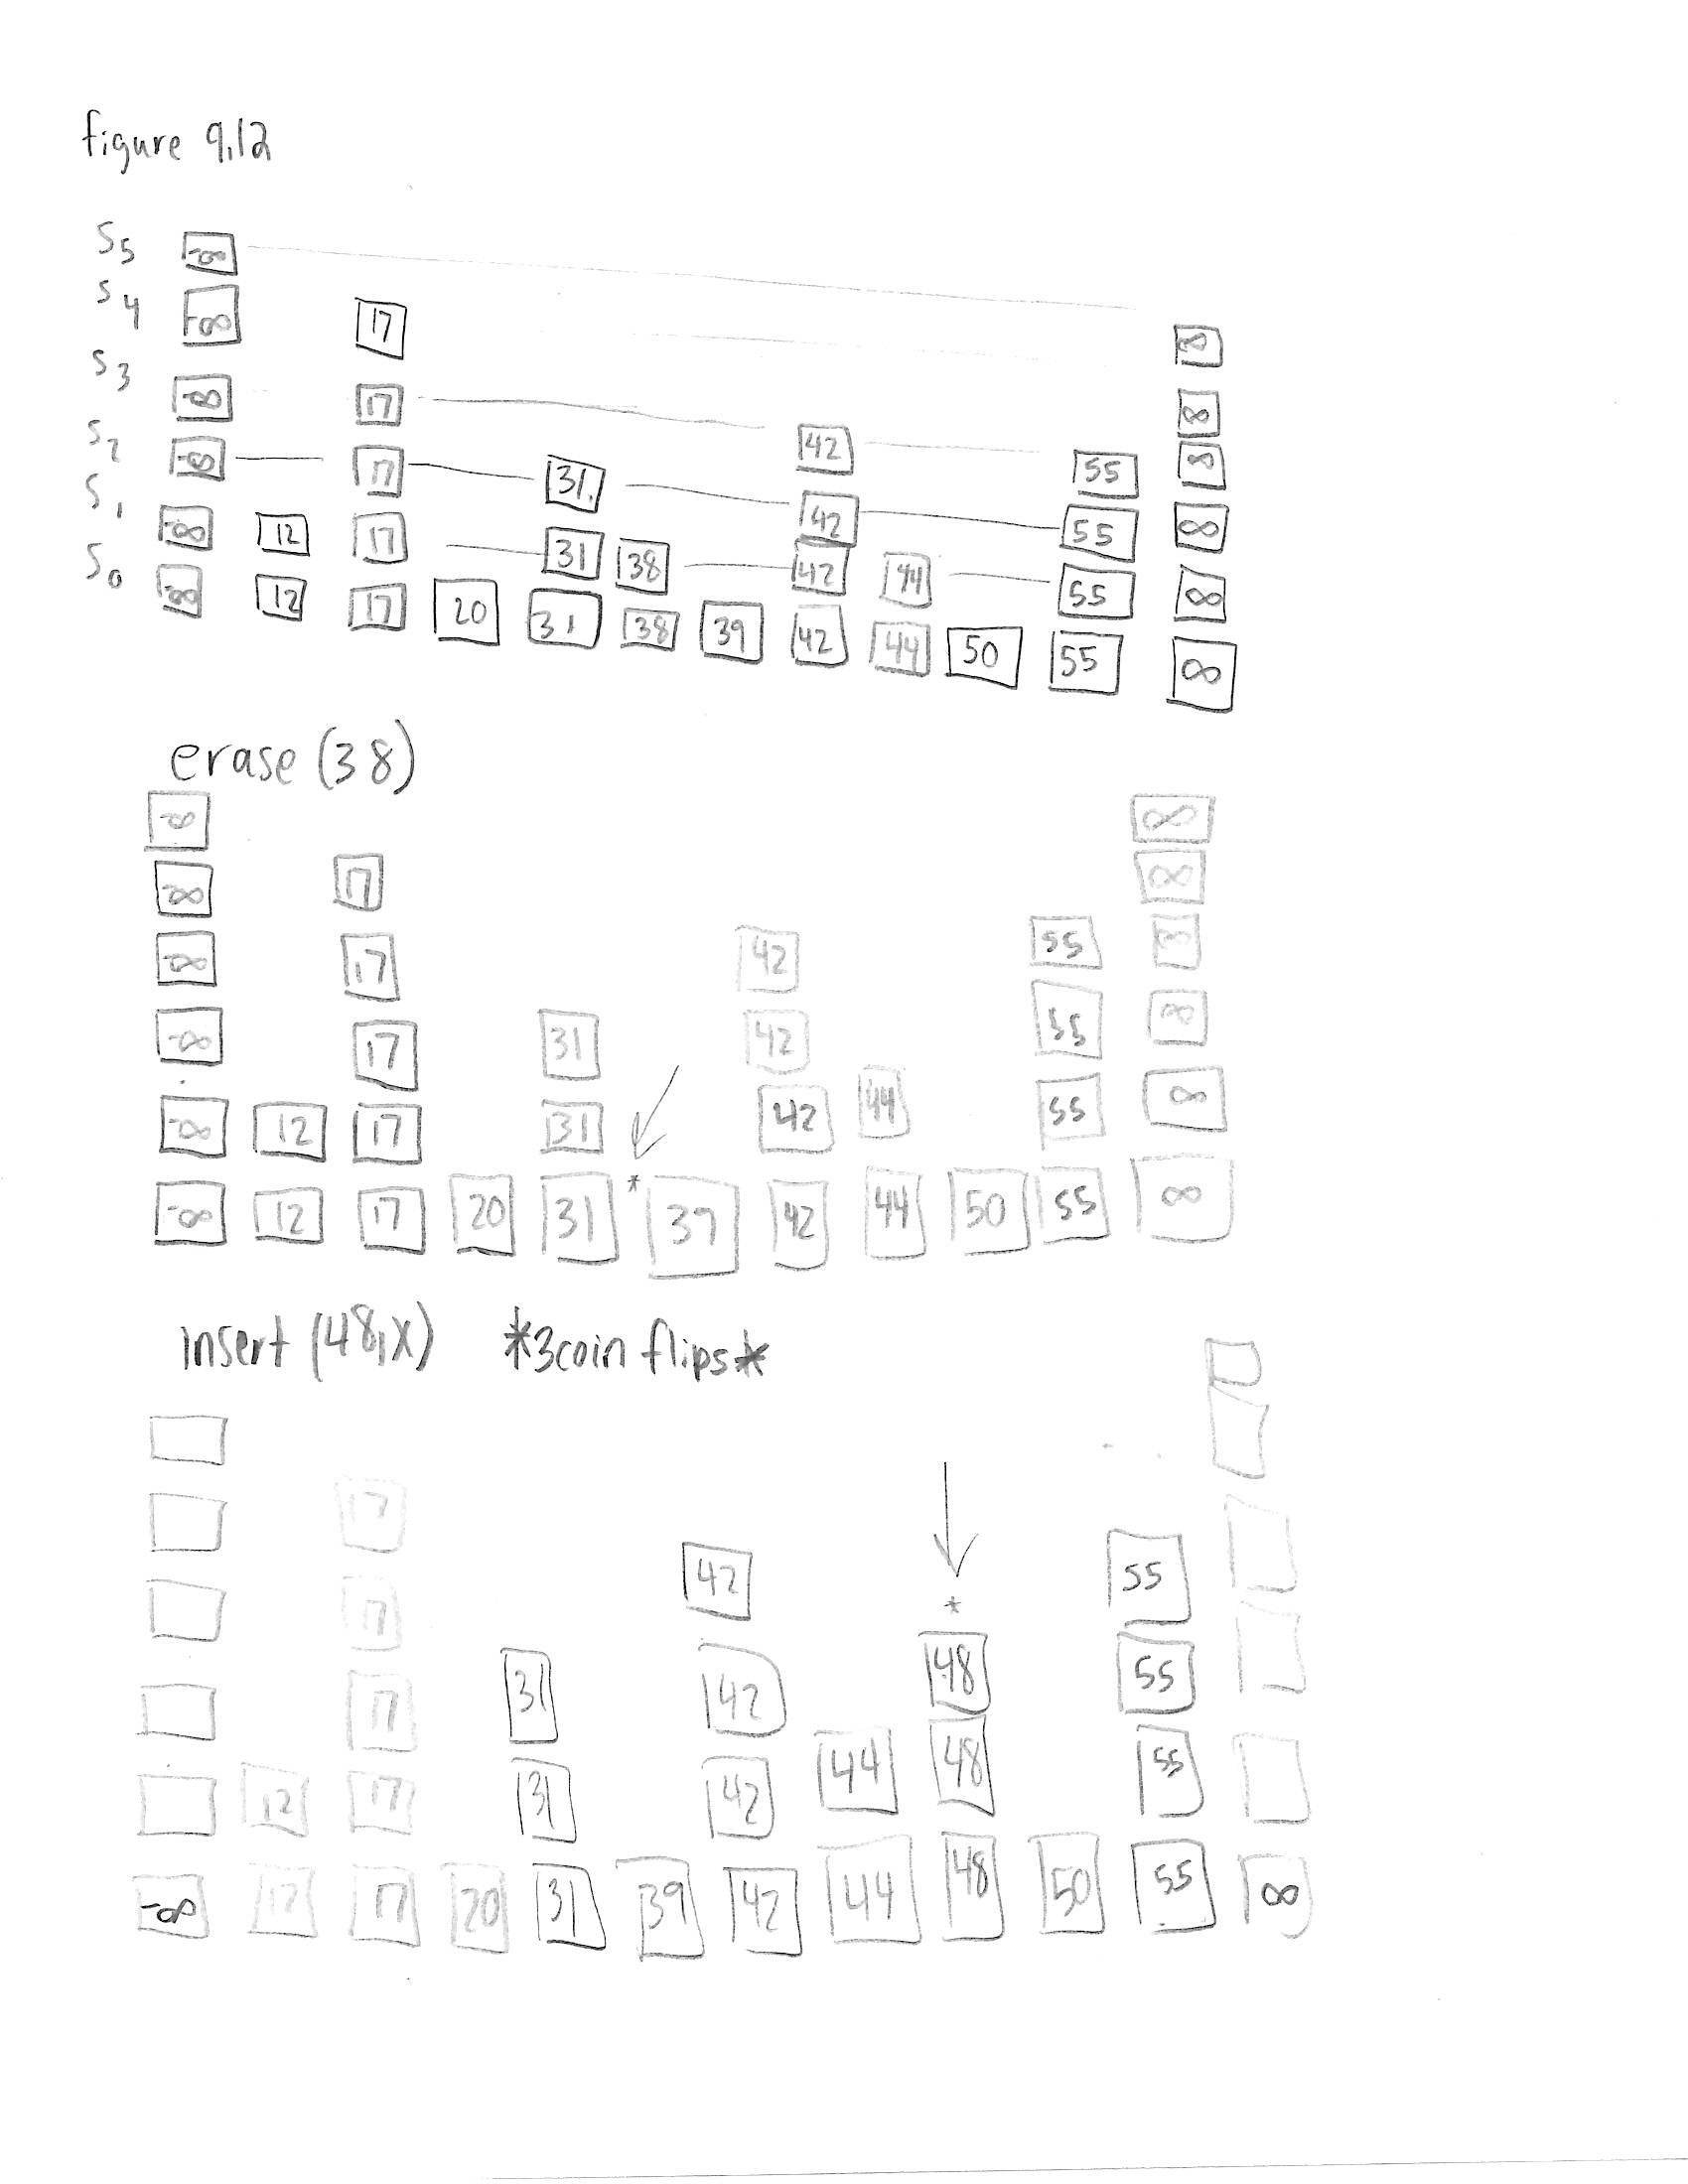
\includegraphics[width=12cm,height=\textheight,keepaspectratio]{EPSON007.JPG}\ \\
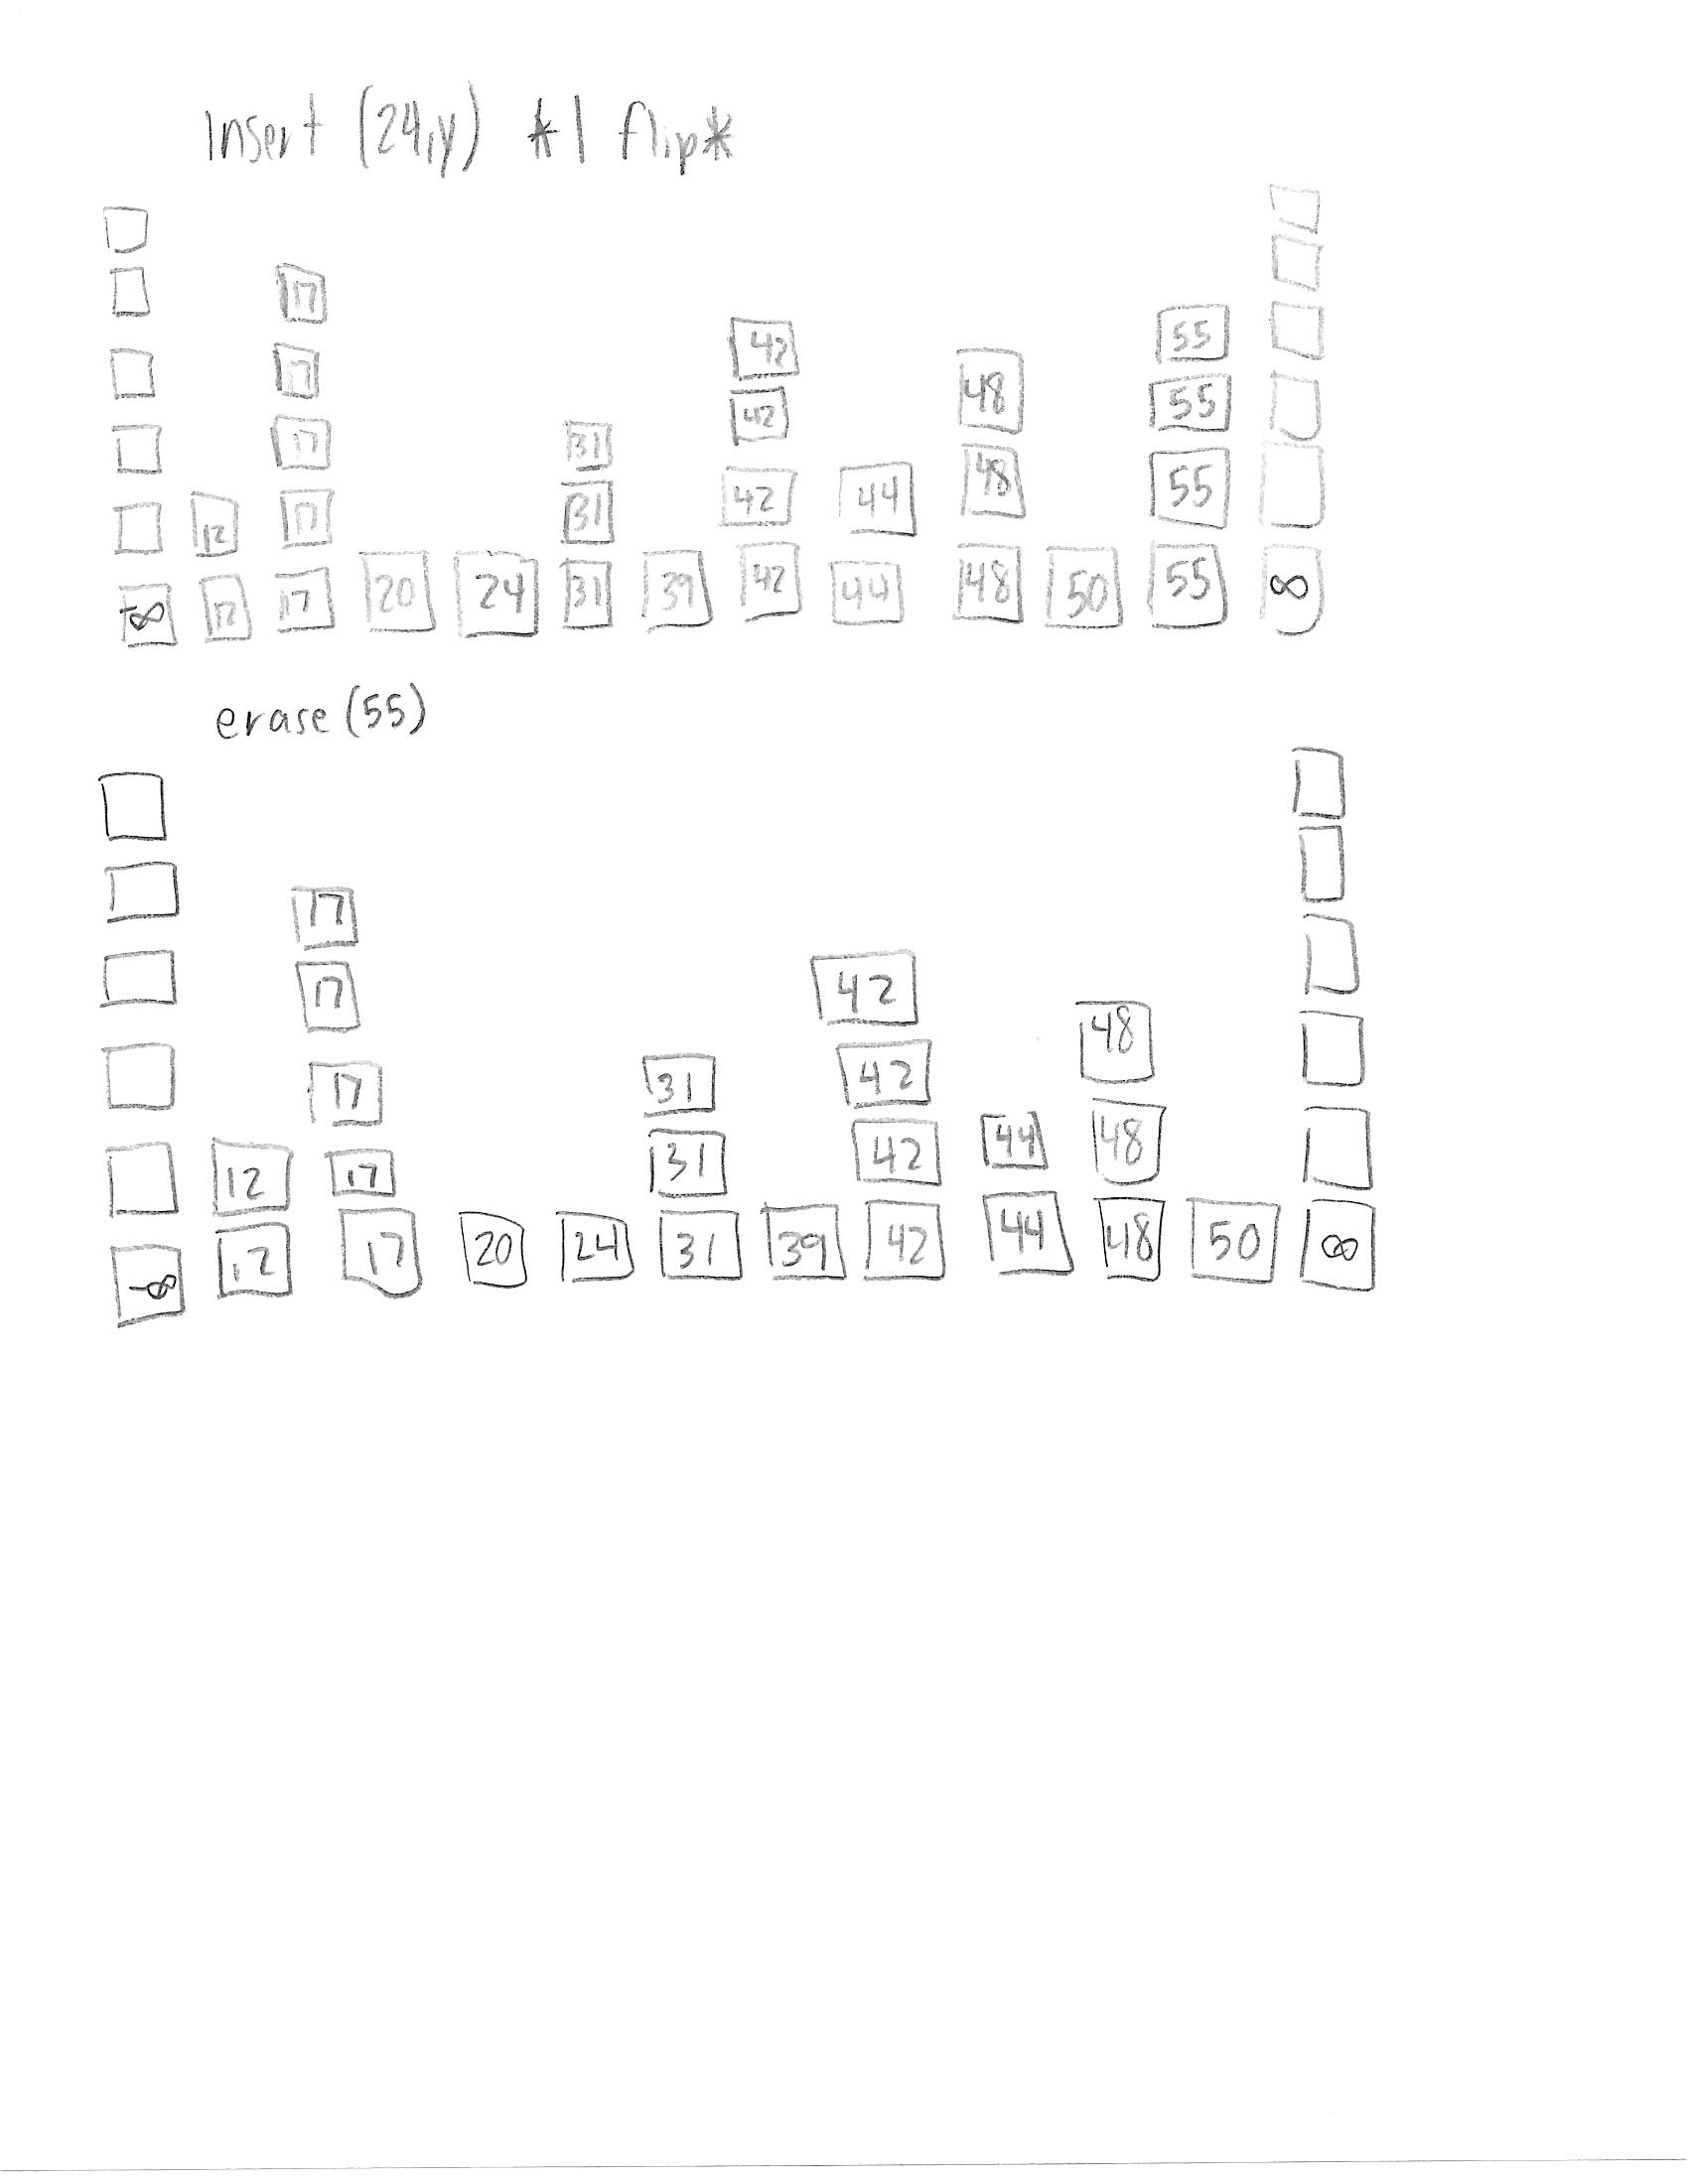
\includegraphics[width=12cm,height=\textheight,keepaspectratio]{EPSON008.JPG}\ \\
\end{enumerate}

\end{document}
